% changelog: "0.1.0 & 2024-04-12 & Stesura sezione "Modello di Sviluppo" e inizio sezione "Organigramma".
\documentclass[8pt]{article}
\usepackage[italian]{babel}
\usepackage[utf8]{inputenc}
\usepackage[letterpaper, left=1in, right=1in, bottom=0.75in, top=0.75in]{geometry}
\usepackage{amsmath}
\usepackage{subfiles}
\usepackage{lipsum}
\usepackage{csquotes}
\usepackage{amsfonts}
\usepackage[sfdefault]{plex-sans}
\usepackage{float}
\usepackage{pifont}
\usepackage{mathabx}
\usepackage[euler]{textgreek}
\usepackage{makecell}
\usepackage{tikz}
\usepackage{wrapfig}
\usepackage{siunitx}
\usepackage{amssymb} 
\usepackage{tabularx}
\usepackage{adjustbox}
\usepackage[document]{ragged2e}
\usepackage{floatflt}
\usepackage[hidelinks]{hyperref}
\usepackage{graphicx}
\usepackage{hyperref}
\setcounter{tocdepth}{4}
\usepackage{caption}
\usepackage{multicol}
\usepackage{tikz}
\setlength\parindent{0pt}
\captionsetup{font=footnotesize}
\usepackage{fancyhdr} 
\usepackage{graphicx}
\usepackage{capt-of}% 
\usepackage{booktabs}
\usepackage{varwidth}

% -- TITOLO INTESTAZIONE -- %
\newcommand{\customtitle}{Piano di Progetto} % o ESTERNO

% -- STILE INTESTAZIONE -- %
\fancypagestyle{mystyle}{
	\fancyhf{} 
	\fancyhead[R]{
\includegraphics[height=1cm]{../../template/images/logos/NaN1fy_logo.png}} 
	\fancyhead[L]{\leftmark} 
	\renewcommand{\headrulewidth}{1pt} 
	\fancyhead[L]{\customtitle} 
	\renewcommand{\headsep}{1.3cm} 
	\fancyfoot[C]{\thepage} 
}

% -- PER LA FIRMA -- %
\newcommand{\signatureline}[1]{%
	 \par\vspace{0.5cm}
	\noindent\makebox[\linewidth][r]{\rule{0.2\textwidth}{0.5pt}\hspace{3cm}\makebox[0pt][r]{\vspace{3pt}\footnotesize #1}}%
}

% -- PER IL GLOSSARIO -- %
\newcommand{\glossterm}[1]{#1\textsuperscript{G}} % inserisci \glossterm{termine}

\begin{document}
\definecolor{myblue}{RGB}{23,103,162}
\begin{titlepage}
	\begin{tikzpicture}[remember picture, overlay]
		\node[anchor=south east, opacity=0.2, yshift = -4cm, xshift= 2em] at (current page.south east) {
\includegraphics[width=0.7\textwidth, trim=0cm 0cm 5cm 0cm, clip]{../../template/images/logos/Universita_Padova_transparent.png}}; 
		\node[anchor=north west, opacity=1, yshift = 4.2cm, xshift= 1.4cm, scale=1.6] at (current page.south west) {
\includegraphics[width=4cm]{../../template/images/logos/NaN1fy_logo.png}};
	\end{tikzpicture}
	
	\begin{minipage}[t]{0.47\textwidth}
		{\large{\textsc{Destinatari}}
			\vspace{3mm}
			\\ \large{\textsc{Prof. Tullio Vardanega}}
			\\ \large{\textsc{Prof. Riccardo Cardin}}
		}
	\end{minipage}
	\hfill
	\begin{minipage}[t]{0.47\textwidth}\raggedleft
		{\large{\textsc{Redattori}}
			\vspace{3mm}
			{\\\large{\textsc{Linda Barbiero}\\}} % massimo due 
			% {\large{\textsc{XXXX XXXX}}}
			
			
		}
		\vspace{8mm}
		
		{\large{\textsc{Verificatori}}
			\vspace{3mm}
			{\\\large{\textsc{XXXX XXXX}\\}} % massimo due 
			{\large{\textsc{XXXX XXXX}}}
			
		}
		\vspace{4mm}\vspace{4mm}
	\end{minipage}
	\vspace{4cm}
	\begin{center}
		\begin{flushright}
			{\fontsize{30pt}{52pt}\selectfont \textbf{Piano di Progetto\\}} % o ESTERNO
		\end{flushright}
		\vspace{3cm}
	\end{center}
	\vspace{8 cm}
	{\small \textsc{\href{mailto: nan1fyteam.unipd@gmail.com}{nan1fyteam.unipd@gmail.com}}}
\end{titlepage}
\pagestyle{mystyle}
\section*{Registro delle Modifiche}
\begin{table}[ht!]	
	\centering
	\begin{tabular}{p{1.2cm} p{2cm} p{6cm} p{3cm} p{2cm}}
		\toprule
		\textbf{Versione}& \textbf{Data} & \textbf{Descrizione} & \textbf{Autore} & \textbf{Ruolo} \\
		\midrule
		0.1.0 & 2024-04-12 & Stesura sezione "Modello di Sviluppo" e inizio sezione "Organigramma". & Linda Barbiero & Progettista \\\\
		0.0.0 & 2024-04-12 & Stesura del file e sezione "Pianificazione". & Linda Barbiero &
		Progettista \\\\ % spazio tra le righe
		% X.X.X & YYYY-MM-DD & Lorem ipsum dolor sit amet, consectetur adipiscing elit.  & XXXX XXXX & --- \\
		\bottomrule
		% Ruolo Redattore o Verificatore
	\end{tabular}
	\caption{Registro delle modifiche.}
	\label{table:Registro delle modifiche}
\end{table}
\newpage
\tableofcontents
\clearpage
\newpage
\justifying
\section{Introduzione}
\section{Analisi dei Rischi}
Sono molteplici gli imprevisti che si possono manifestare durante la realizzazione di un progetto. Se non affrontate correttamente, le problematiche riscontrate possono impattare negativamente sullo svolgimento delle attività, causando un aumento dei costi, ritardi nel processo di sviluppo e una diminuzione della \glossterm{qualità} del prodotto. Pertanto, si rivela essenziale condurre un'analisi approfondita dei rischi che possono insorgere, con l'obiettivo di prevenirli o quantomeno attenuarne gli effetti. \\
Il \glossterm{processo} di mitigazione si compone quindi delle seguenti fasi: 
\begin{itemize}
\setlength\itemsep{0em}
    \item \textbf{Identificazione:} individuazione della minaccia, riconoscendone origine e contesto d'insorgenza;
    \item \textbf{Valutazione:} stima della probabilità di occorrenza e assegnazione di un grado di pericolosità indicativo del potenziale impatto sul progetto;
    \item \textbf{Mitigazione:} adozione di strategie di prevenzione e contrasto delle possibili conseguenze negative derivanti da una situazione avversa.
\end{itemize}
Per garantire uno svolgimento efficiente del progetto è necessario compiere un monitoraggio periodico delle attività, in modo da riconoscere eventuali nuovi rischi o aggiornare un processo di mitigazione precedentemente definito. \\ Di seguito sono elencati i rischi individuati, suddivisi per contesto d'insorgenza.

\subsection{Rischi tecnologici}
\subsubsection{RT-1 Inesperienza}
La scarsa conoscenza delle tecnologie richieste per la realizzazione del prodotto determina la necessità di formazione preliminare alle fasi di progettazione e sviluppo, con conseguenti possibili ritardi.
\begin{itemize}
\setlength\itemsep{0em}
    \item \textbf{Identificazione:} ciascun membro del gruppo ha notificato il proprio grado di conoscenza delle tecnologie richieste dal \glossterm{capitolato} agli altri componenti e alla \glossterm{Proponente}. In questo modo è stato più semplice desumere i punti di forza del fornitore e gli argomenti che invece avrebbero necessitato di maggiori approfondimenti;
    \item \textbf{Valutazione:} pericolosità: alta; probabilità: alta;
    \item \textbf{Mitigazione:} la Proponente si è resa disponibile ad assistere il team nell'apprendimento di alcune tecnologie, grazie ad incontri dedicati e al sostegno di una figura competente in grado di fornire supporto tecnico. In aggiunta, il gruppo organizzerà dei \textit{workshop} interni, oltre a prevedere il lavoro di coppia per lo svolgimento di determinati compiti. L'aiuto reciproco e la condivisione delle conoscenze rendono infatti più efficiente il \glossterm{processo} di formazione e aiutano a rafforzare lo spirito di squadra.
\end{itemize}

\subsubsection{RT-2 Produzione di codice incomprensibile}
La partecipazione alla stesura del codice sorgente da parte di diversi membri del gruppo, ciascuno con il proprio grado di esperienza e stile di programmazione, può portare alla produzione di codice difficilmente leggibile, il quale può generare fraintendimenti ed essere sintomo di scarsa \glossterm{qualità} del prodotto. 
\begin{itemize}
\setlength\itemsep{0em}
    \item \textbf{Identificazione:} questa problematica si manifesta quando risulta difficoltoso interpretare il codice scritto da altri componenti, al punto da causare un aumento di discussioni interne;
    \item \textbf{Valutazione:} pericolosità: media; probabilità: media;
    \item \textbf{Mitigazione:} saranno adottate delle convenzioni di codifica con l'obiettivo di rendere omogeneo e maggiormente manutenibile il codice prodotto. Esso sarà inoltre corredato dell'adeguata documentazione e soggetto a revisioni continue.
\end{itemize}

\subsubsection{RT-3 Perdita delle informazioni}
I file contenenti la documentazione ed il codice sorgente potrebbero essere soggetti a danneggiamento a causa di errori umani o malfunzionamenti hardware, inficiando così il normale proseguimento del lavoro.
\begin{itemize}
\setlength\itemsep{0em}
    \item \textbf{Identificazione:} il rischio si concretizza nel momento in cui si verifica un guasto, si effettuano modifiche indesiderate o si eliminano accidentalmente i file del progetto;
    \item \textbf{Valutazione:} pericolosità: alta; probabilità: bassa;
    \item \textbf{Mitigazione:} i file sono mantenuti in una \glossterm{repository} remota, in modo garantire a tutti i membri del gruppo la possibilità di accedervi agevolmente e preservarli da eventuali malfunzionamenti dei singoli dispositivi. Inoltre, viene adottato un sistema di \glossterm{versionamento} per consentire il recupero di versioni precedenti, proteggendo così i documenti da alterazioni sgradite dovute ad errori umani. 
\end{itemize}

\subsection{Rischi di comunicazione}
\subsubsection{RC-1 Scarsa comunicazione interna}
Una comunicazione interna inefficace può causare fraintendimenti e disorganizzazione, generando tensione e sconforto tra i componenti del gruppo. Questa problematica impatta ovviamente anche sull'adeguato proseguimento delle attività, che potrebbe infatti subire significativi ritardi.
\begin{itemize}
\setlength\itemsep{0em}
    \item \textbf{Identificazione:} l'eccessiva durata delle riunioni interne, la reiterazione di questioni già affrontate in precedenza e incomprensioni frequenti suggeriscono l'occorrenza di questa complicazione;
    \item \textbf{Valutazione:} pericolosità: alta; probabilità: bassa;
    \item \textbf{Mitigazione:} la prevenzione di questo rischio è messa in atto grazie all'utilizzo di diversi canali di comunicazione, all'organizzazione di incontri periodici, alla definizione anticipata dell'ordine del giorno delle riunioni e alla produzione di documentazione adeguata per tenere traccia delle decisioni prese e delle discussioni affrontate.
\end{itemize}

\subsubsection{RC-2 Scarsa comunicazione con la \glossterm{Proponente}}
Comunicare con la Proponente in modo sporadico e disorganizzato potrebbe compromettere significativamente la \glossterm{qualità} del prodotto realizzato. Inoltre, l'azienda ricopre il ruolo di mentore del gruppo, dunque svolgere le attività previste senza un adeguato supporto può provocare caos e smarrimento.
\begin{itemize}
\setlength\itemsep{0em}
    \item \textbf{Identificazione:} sintomi di questa problematica sono la riproposizione dei medesimi quesiti alla proponente da parte del gruppo fornitore e incomprensioni riguardanti le aspettative sul prodotto da realizzare;
    \item \textbf{Valutazione:} pericolosità: alta; probabilità: bassa;
    \item \textbf{Mitigazione:} si terranno incontri periodici per verificare lo stato di avanzamento del lavoro (\glossterm{SAL}). La proponente ha inoltre predisposto un canale di messaggistica istantanea, in aggiunta alla comunicazione via mail, per chiarire i dubbi che insorgono durante lo svolgimento delle attività assegnate.
\end{itemize}

\subsubsection{RC-3 Conflitti interni}
Durante lo svolgimento del progetto potrebbero sorgere dei contrasti dovuti alla diversità di opinioni, con il rischio di influire negativamente sulla capacità decisionale del gruppo, rallentando così il proseguimento delle attività.
\begin{itemize}
\setlength\itemsep{0em}
    \item \textbf{Identificazione:} il problema si manifesta quando, osservando le dinamiche interne al gruppo, si riconoscono tensioni tra i membri, si verificano discussioni ripetute e vi è una diffusa diffidenza;
    \item \textbf{Valutazione:} pericolosità: media; probabilità: bassa;
    \item \textbf{Mitigazione:} a ciascun membro del team viene offerto lo spazio sufficiente per esprimere le proprie idee ed avanzare nuove proposte. Ciascuna iniziativa diverrà poi oggetto di discussione interna, la quale si concluderà con una votazione. Affinché il confronto avvenga sempre in modo rispettoso e sia garantito il raggiungimento di una soluzione concreta in tempi ragionevoli, il responsabile assumerà il ruolo di mediatore, supervisionando i dibattiti con l'obiettivo di trovare un accordo soddisfacente.
\end{itemize}

\subsubsection{RC-4 Confusione nella rotazione dei ruoli}
La mancanza di chiarezza sui ruoli ricoperti e sulle responsabilità assunte da ciascuna componente del gruppo può impattare negativamente sull'organizzazione delle attività e generare conflitti interni.
\begin{itemize}
\setlength\itemsep{0em}
    \item \textbf{Identificazione:} si riscontrano frequentemente perplessità sul lavoro svolto sino a quel momento, dovute ad una pianificazione disordinata oppure ad una comunicazione scarsa o ambigua;
    \item \textbf{Valutazione:} pericolosità: media; probabilità: media;
    \item \textbf{Mitigazione:} è necessario definire chiaramente le responsabilità di ciascuno ancor prima di cimentarsi nello svolgimento delle attività. Successivamente, è indispensabile che ogni membro comprenda come ricoprire il proprio ruolo nella maniera più consona. Pertanto, la persona che ha svolto la medesima funzione nello \glossterm{Sprint} precedente condividerà le conoscenze acquisite con il suo successore, al fine di facilitare l'apprendimento degli incarichi assegnati.
\end{itemize}

\subsection{Rischi di pianificazione}
\subsubsection{RP-1 Stima errata delle tempistiche di progetto}
Al momento del calcolo del preventivo iniziale il gruppo non ha un livello di esperienza tale da consentire una stima accurata del tempo necessario al raggiungimento delle \glossterm{milestone} del progetto. La previsione potrebbe quindi rivelarsi inesatta, portando, nel peggiore dei casi, ad un considerevole ritardo nello svolgimento del progetto.
\begin{itemize}
\setlength\itemsep{0em}
    \item \textbf{Identificazione:} questa complicazione si verifica quando risulta evidente che la data prevista per il raggiungimento di una milestone differisce significativamente dalla data di effettivo completamento delle attività relative alla suddetta milestone;
    \item \textbf{Valutazione:} pericolosità: alta; probabilità: media;
    \item \textbf{Mitigazione:} aggiornamenti frequenti sull'avanzamento del progetto permettono di adottare una pianificazione flessibile. Le attività sono quindi di volta in volta pianificate con l'obiettivo di rispettare i tempi stabiliti.
\end{itemize}

\subsubsection{RP-2 Stima errata dei costi di progetto}
Al momento del calcolo del preventivo iniziale il gruppo non ha un livello di esperienza tale da consentire una stima accurata e realistica dei costi, che potrebbero quindi subire variazioni impreviste.
\begin{itemize}
\setlength\itemsep{0em}
    \item \textbf{Identificazione:} una manifestazione lampante di questa problematica è un eccessivo divario tra preventivo e consuntivo, riscontrabile grazie ad un confronto con quanto riportato nel \textit{Piano di Progetto};
    \item \textbf{Valutazione:} pericolosità: alta; probabilità: media;
    \item \textbf{Mitigazione:} il calcolo del preventivo ad ogni \glossterm{Sprint} e la corrispondente rendicontazione del consuntivo di periodo permettono di maturare accuratezza nelle previsioni e monitorare i costi effettivi. La proponente viene informata periodicamente di eventuali variazioni.
\end{itemize}

\subsubsection{RP-3 Stima errata del tempo di completamento di un'attività}
La sottostima o la sovrastima del tempo necessario per lo svolgimento di un incarico possono portare rispettivamente allo slittamento delle attività già pianificate o all'attesa superflua per il proseguimento del lavoro. Entrambe gli errori di valutazione possono provocare ritardi nello sviluppo.
\begin{itemize}
\setlength\itemsep{0em}
    \item \textbf{Identificazione:} questo rischio si concretizza quando, durante le retrospettive sul lavoro svolto, si notano discrepanze tra l'intervallo temporale preventivato per lo svolgimento di un singolo compito e le ore effettivamente impiegate;
    \item \textbf{Valutazione:} pericolosità: media; probabilità: alta;
    \item \textbf{Mitigazione:} aggiornamenti frequenti sull'avanzamento del progetto permettono di adottare una pianificazione flessibile. Il Responsabile può quindi assegnare maggiori risorse ad attività che si rivelano essere più onerose del previsto e viceversa. In aggiunta, la ripetizione in ogni Sprint dell'attività di valutazione delle tempistiche consente di sviluppare maggiore precisione, producendo man mano stime sempre più realistiche.
\end{itemize}

\subsubsection{RP-4 Variazione requisiti di progetto}
La possibilità i requisiti cambino in corso d'opera può comportare la necessità di revisione della pianificazione iniziale e l'adeguamento del lavoro svolto alle nuove richieste, causando ritardi e aumenti dei costi.
\begin{itemize}
\setlength\itemsep{0em}
    \item \textbf{Identificazione:} la \glossterm{Proponente} comunica al fornitore nuove esigenze, differenti da quanto riferito in precedenza. Ciò si traduce in modifiche da apportare a quanto già prodotto o aggiunte non previste;
    \item \textbf{Valutazione:} pericolosità: alta; probabilità: bassa;
    \item \textbf{Mitigazione:} il team viene aggiornato regolarmente dalla Proponente grazie a comunicazioni chiare ed opportunamente frequenti. L'azienda ha modo di constatare la conformità del prodotto alle aspettative descritte mediante incontri periodici di revisione dell'operato (\glossterm{SAL}).
\end{itemize}

\subsubsection{RP-5 Impegni personali ed accademici}
Durante le settimane predisposte allo svolgimento del progetto i componenti del gruppo potrebbero imbattersi in alcuni impedimenti esterni indeclinabili, quali esami universitari, problemi di salute o altre tipologie di incombenze. 
Ciò può indurre a diminuire il quantitativo di ore dedicate all'esecuzione delle attività previste, con conseguenti rallentamenti.
\begin{itemize}
\setlength\itemsep{0em}
    \item \textbf{Identificazione:} ciascuno notifica al team i propri impegni nel momento in cui viene a conoscenza della loro occorrenza;
    \item \textbf{Valutazione:} pericolosità: media; probabilità: bassa;
    \item \textbf{Mitigazione:} per ovviare alle conseguenze negative di questo rischio è utile effettuare una pianificazione delle attività che tenga in considerazione gli impegni inevitabili di ognuno. Pertanto, se dovesse rivelarsi necessario, le ore di lavoro assegnate durante i periodi di disponibilità limitata possono essere ridotte, ricollocando di conseguenza le scadenze prefissate. 
\end{itemize}

\subsection{Tabella riassuntiva}
Segue una sintesi dei rischi sopracitati, riportandone in particolare il grado di pericolosità e la probabilità di occorrenza.

\begin{table}[ht!]
    \centering
    \renewcommand{\arraystretch}{1.25}
    \begin{tabular}{cccc}
        \toprule
        \textbf{Codice} & \textbf{Rischio} & \textbf{Pericolosità} & \textbf{Probabilità} \\ \midrule
        RT-1 & Inesperienza & Alta & Alta \\ 
        RT-2 & Produzione di codice incomprensibile & Media & Media \\ 
        RT-3 & Perdita delle informazioni & Alta & Bassa \\ 
        RC-1 & Scarsa comunicazione interna & Alta & Bassa \\ 
        RC-2 & Scarsa comunicazione con la \glossterm{Proponente} & Alta & Bassa \\ 
        RC-3 & Conflitti interni & Media & Bassa \\ 
        RC-4 & Confusione nella rotazione dei ruoli & Media & Media \\ 
        RP-1 & Stima errata delle tempistiche di progetto & Alta & Media \\ 
        RP-2 & Stima errata dei costi di progetto & Alta & Media \\ 
        RP-3 & Stima errata del tempo di completamento di un'attività & Media & Alta \\ 
        RP-4 & Variazione requisiti di progetto & Alta & Bassa \\ 
        RP-5 & Impegni personali ed accademici & Media & Bassa \\ 
        \bottomrule
    \end{tabular}
    \caption{Tabella riassuntiva dei rischi.}
    \label{table:Tabella riassuntiva dei rischi}
\end{table}
\newpage

\section{Modello di Sviluppo}
\subsection{Modello Agile}
Un approccio metodologico agile fornisce un insieme di caratteristiche che lo rendono particolarmente idoneo per gestire le tempistiche limitate di rilascio, garantendo comunque un progetto di qualità buona.
Questa metodologia prevede la realizzazione di molteplici rilasci successivi, ciascuno dei quali porta con sé un incremento delle funzionalità. Adottando tale approccio, diventa essenziale identificare e classificare i requisiti in modo da definire un ordine di priorità nello sviluppo, consentendo di ottenere, dopo ogni incremento, un prodotto stabile e funzionante, seppur incompleto. Per garantire la stabilità del prodotto sin dalle prime fasi, è cruciale che i primi incrementi soddisfino i requisiti più significativi, mentre quelli di minore importanza saranno integrati in un secondo momento, permettendo loro di stabilizzarsi gradualmente nel contesto del prodotto.
\\\\
I vantaggi da evidenziare sono i seguenti:
\begin{itemize}
\setlength\itemsep{0em}
\item
\textbf{\emph{Iterazioni rapide}}: Sprint brevi e frequenti permettono di ottenere risultati tangibili in tempi rapidi e di adattare il piano di sviluppo in base ai feedback e alle esigenze emergenti.
\item
\textbf{\emph{Flessibilità e adattabilità}}: Si portanno apportare modifiche al prodotto anche in corso d'opera senza dover ripensare completamente il \textit{Piano di Progetto}.
\item
\textbf{\emph{Coinvolgimento del cliente / proponente}}: Permette il coinvolgimento col proponente continuo durante tutto il ciclo di sviluppo, così da avere feedback tempestivi e garantire che il prodotto finale soddisfi effettivamente le esigenze.
\item
\textbf{\emph{Focus sulla qualità}}: La pratica di sviluppo incrementale, al testing continuo e al coinvolgimento degli stakeholder consente comunque di mantere alta la qualità del software.
\item
\textbf{\emph{Comunicazione e collaborazione}}: I membri del team rimangono allineati sugli obiettivi e sulle priorità del progetto, riducendo i rischi di fraintendimenti e conflitti.
\end{itemize}
\section{Pianificazione}
\subsection{Scadenze}
\begin{itemize}
\setlength\itemsep{0em}
    \item RTB (Requirements and Technology Baseline) : 2024-06-07;
    \item PB (Product Baseline) : 2024-07-26;
    \item CA (Customer Acceptance) : 2024-08-09.
\end{itemize}
\subsection{Verso la RTB}
\textit{Periodo: dal 2024-04-01 al 2024-06-07}
\newpage
\subsubsection{Primo periodo}
\textit{Periodo: dal 2024-04-01 al 2024-04-19}
\\\\
Nella fase iniziale, assume prioritaria importanza la discussione di tutte le regole precedentemente adottate e implementate nel corso del progetto, ma che non sono ancora state formalizzate mediante documentazione. Questo processo mira a produrre un documento scritto accessibile a tutti i membri del team, al fine di dissipare eventuali ambiguità riguardo l'esecuzione delle attività e l'utilizzo delle risorse.
\\
Inoltre, durante questa fase, è cruciale identificare tutti i potenziali rischi che potrebbero ostacolare il progresso del progetto, al fine di prevenirli e non essere colti impreparati. Un'altra priorità consiste nell'avviare la pianificazione delle prime attività e delle relative milestone, al fine di organizzare le risorse disponibili e fornire una stima preventiva dei tempi e dei costi.
\\
\begin{figure}[h]
    \centering
    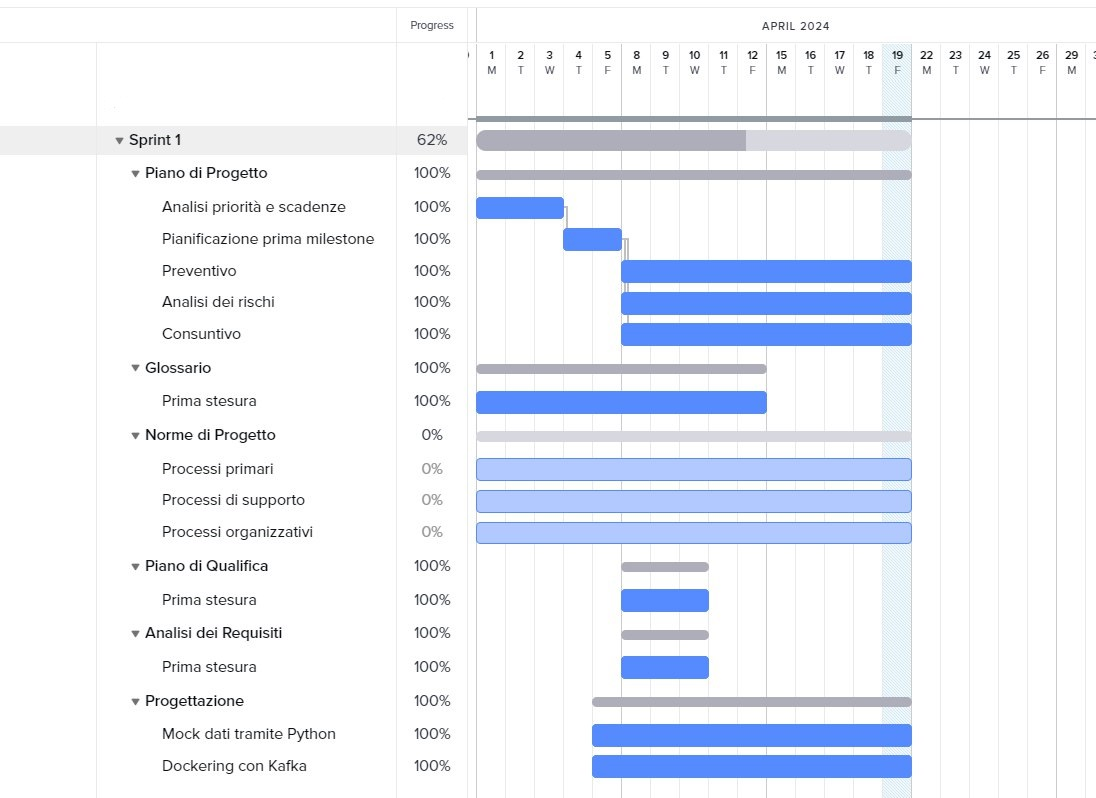
\includegraphics[width=15cm]{./asset/gantt1.jpeg}
    \caption{Diagramma di Gantt rappresentativo del primo periodo}
    \label{figure:Diagramma di Gantt rappresentativo del primo periodo}
\end{figure}
\subsubsection{Secondo periodo}
\textit{Periodo: dal 2024-04-22 al 2024-05-03}
\\\\
In questa fase del processo, assume un'importanza fondamentale condurre un'analisi dettagliata del capitolato al fine di identificare accuratamente i casi d'uso necessari. Inoltre, al fine di evitare ambiguità e decisioni errate, si raccomanda di organizzare uno o più incontri con il proponente per condividere le idee e risolvere i dubbi emersi durante l'analisi, che sarà notevolmente più approfondita rispetto a quella svolta durante la selezione del capitolato.
Da questo processo di analisi, si darà inizio alla stesura dell'\textit{Analisi dei Requisiti}, un documento di vitale importanza per il progetto poiché conterrà tutti i casi d'uso individuati, nonché i requisiti obbligatori, desiderabili e opzionali.
È altresì consigliabile redigere il \textit{Piano di Qualifica} in questa fase, il quale sarà fondamentale per definire i metodi volti a garantire la qualità dei processi e dei prodotti nel corso dello sviluppo.

\begin{figure}[h]
    \centering
    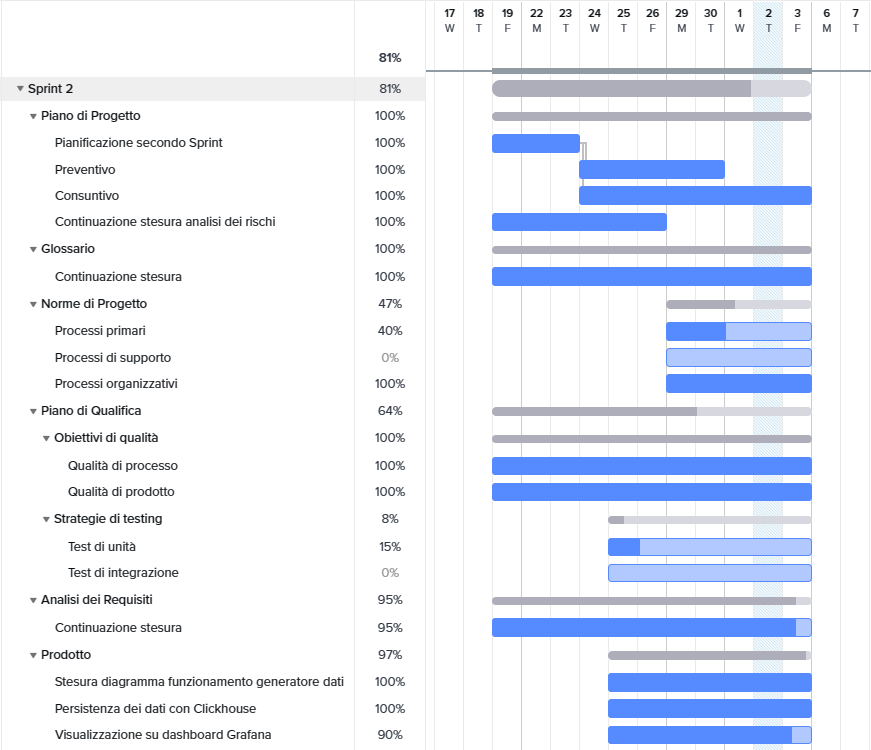
\includegraphics[width=13cm]{./asset/gantt2.png}
    \caption{Diagramma di Gantt rappresentativo del secondo periodo}
    \label{figure:Diagramma di Gantt rappresentativo del secondo periodo}
\end{figure}

\subsubsection{Terzo periodo}
\textit{Periodo: dal 2024-04-29 al 2024-05-17}
Con la completamento dell'\textit{Analisi dei Requisiti}, assume un ruolo cruciale l'approfondimento delle tecnologie e degli strumenti necessari per l'implementazione del prodotto. Questo processo consentirà la realizzazione del \textit{PoC} (Proof of Concept), una versione semplificata del prodotto finale che mira a fornire indicazioni sulla validità della direzione intrapresa e a dimostrare al committente la correttezza dell'approccio di sviluppo.

\subsubsection{Quarto periodo}
\textit{Periodo: dal 2024-05-20 al 2024-06-07}
\\\\
In questa fase conclusiva del processo, assume primaria importanza sia la progettazione che l'effettiva implementazione del \textit{PoC}. Parallelamente, diventa imprescindibile il perfezionamento e la verifica finale dei documenti in vista della revisione pianificata per l'inizio del mese di giugno.

\subsection{Verso la PB}
\textit{Periodo: dal 2024-06-08 al 2024-07-26}
\\\\
Superata la prima revisione, l'obiettivo principale è realizzare una prima versione del prodotto finale che dimostri come ha già fatto il \textit{PoC}, nella sua semplicità, 
che requisiti e tecnologie scelte possono coesistere nello stesso prodotto. 
\\
Sarà, quindi, fondamentale la progettazione per arrivare ad avere un design che sia quello definitivo e poi avere un avanzamento consistente di codifica e verifica.

\subsection{Verso la CA}
\textit{Periodo: 2024-07-26 - 2024-08-09}
\\\\
Superata la seconda revisione, l'obiettivo rimane quello di presentare al proponente il prodotto finale.
\section{Preventivo}
\subsection{Verso la RTB}
\subsubsection{Primo periodo}
\textbf{Preventivo Orario}
\begin{table}[ht!]
	\centering
	\begin{tabular}{p{4cm} p{1cm} p{1cm} p{1cm} p{1cm} p{1cm} p{1cm} p{3cm}}
		\toprule
        \textbf{Membro} & \multicolumn{6}{c}{\textbf{Ruoli}} & \textbf{Totale (persona)}\\
		& \textbf{AM} & \textbf{RE} & \textbf{PT} & \textbf{AN} & \textbf{PR} & \textbf{VE}\\
		\midrule
        Linda Barbiero & - & 3 & - & 1 & - & 1 & 5 \\
        Guglielmo Barison & 3 & - & 1 & - & 2.5 & 1 & 7.5\\
        Pietro Busato & 3 & - & 1 & - & 2.5 & 1 & 7.5 \\
        Davide Donanzan & 3 & - & - & 2 & - & 1.5 & 6.5 \\
        Oscar Konieczny & 3 & - & - & - & - & 1 & 4 \\
        Veronica Tecchiati & 3 & - & - & 2 & - & 1 & 6 \\
        \bottomrule
        \textbf{Totale (ruolo)} & 15 & 3 & 2 & 5 & 5 & 6.5 & 36.5 \\
	\end{tabular}
	\caption{Distribuzione delle ore della prima milestone secondo ruolo e membro}
	\label{table:Distribuzione delle ore della prima milestone secondo ruolo e membro}
\end{table}
\newpage
\textbf{Preventivo Economico}
\begin{table}[ht!]
	\centering
	\begin{tabular}{p{4cm} p{1cm} p{2cm}}
        \toprule
        \textbf{Ruolo} & \textbf{Ore} & \textbf{Costo (€)} \\
        \midrule
        Amministratore & 15 & 450 \\
        Responsabile & 3 & 60 \\
        Progettista & 2 & 50 \\
        Analista & 5 & 125 \\
        Programmatore & 5 & 75 \\
        Verificatore & 6.5 & 97.5 \\
        \bottomrule
        \textbf{Totale} & 36.5 & 782.5
    \end{tabular}
    \caption{Preventivo dei costi della prima milestone secondo ruolo}
	\label{table:Preventivo dei costi della prima milestone secondo ruolo}
\end{table}

\subsubsection{Secondo periodo}
\subsubsection{Terzo periodo}
\subsubsection{Quarto periodo}

\subsection{Verso la PB}

\subsection{Verso la CA}
\section{Consuntivo}
\subsection{Verso la RTB}
\subsubsection{Primo periodo}
\subsubsection{Secondo periodo}
\subsubsection{Terzo periodo}
\subsubsection{Quarto periodo}

\subsection{Verso la PB}

\subsection{Verso la CA}

\section{Organigramma}
\subsection{Componenti}
\begin{table}[ht!]
	\centering
	\begin{tabular}{p{3cm} p{3cm}}
		\toprule
		\textbf{Nominativo} & \textbf{Matricola} \\
		\midrule
		Guglielmo Barison & 2042324 \\
		Linda Barbiero &  1220244 \\
		Pietro Busato & 2043688 \\
		Oscar Konieczny & 2042335 \\
		Davide Donanzan & 2034337 \\
		Veronica Tecchiati & 2034309 \\
		\bottomrule
	\end{tabular}
	\caption{Nominativi e matricole NaN1fy.}
	\label{table:Nominativi e matricole NaN1fy}
\end{table}

\section{Mitigazione dei Rischi}
\subsection{Test Mitigazione dei Rischi}

\newpage


% togli il commento per la firma
% \signatureline{Padova, YYYY-MM-DD}
%\signatureline{Padova, YYYY-MM-DD}
\end{document}
